\chapter{YAML}
\label{appendix:yaml}

\glsreset{yaml}

\section{¿Qué es YAML?}

\yaml{} es un formato de serialización de datos creado por Clark Evans, Ingy döt Net y Oren Ben-Kiki en 2001 y que está fuertemente inspirado en lenguajes como \xml{}, C, Python y Perl. A diferencia de \xml{}, la sintaxis de \yaml{} es muy liviana y es muy fácil de interpretar por las personas, de hecho, surgió como una alternativa a \xml{} por considerar a éste un poco \textit{engorroso} de crear documentos y, sobre todo, de leerlos.

Actualmente tiene una amplia aceptación en el mundo de la programación, donde, lenguajes tan populares y conocidos como son: C, Python, \textsc{java}, Ruby, Haskell, JavaScript (y otros tantos más) tienen implementaciones, en forma de librerías externas en algunos casos o incluidas en el propio lenguaje en otros, de un intérprete de \yaml{}. Los usos que se le pueden dar son tan variados que dependen del propio programador y lo que desee hacer con el formato aunque, generalmente, se suele utilizar para crear archivos de configuración que luego los programas pueden leer y modificar las preferencias del mismo; un ejemplo claro lo encontramos en el programa \textit{Jekyll} \cite{web:jekyll}. Éste es un generador de sitios web estáticos (muy popular entre la comunidad de programadores) y que utiliza \yaml{} para pasar datos básicos de configuración al propio programa (\figureref{ejemplo_yaml}).
Encontramos la misma situación en varios programas de renombre como: \textit{Ruby on Rails} \cite{web:ruby-on-rails} o \textit{Symfony} \cite{web:symfony} que son dos aplicaciones que sirven para crear páginas web dinámicas y que utilizan a \yaml{} con el mismo objetivo: configurar las propias aplicaciones.

\begin{figure}
\centering
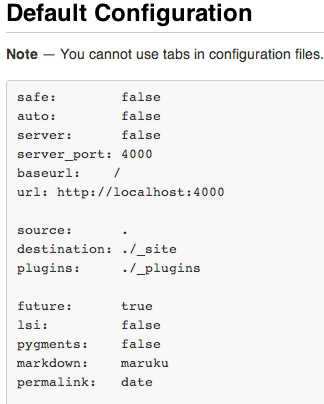
\includegraphics[scale=0.8]{../graphics/fig_ejemplo_yaml.png}
\caption{Ejemplo de configuración del programa Jekyll utilizando \yaml{}.}\label{fig:ejemplo_yaml}
\end{figure}

El hecho de que los \profiles{} utilicen \yaml{} no es otro que por la claridad de lectura que se obtiene con ellos. Además, en el caso de \php{}, hay una implementación del formato incluida en el propio lenguaje que está bastante optimizada.

En la web podemos encontrar multitud de recursos para aprender sobre la especificación de \yaml{}. En este apéndice, en concreto, sólo se mostrarán los elementos más básicos del lenguaje. Si deseamos obtener más información no hay nada mejor que ir a la página oficial \cite{web:especificacion-yaml} donde siempre encontraremos la última versión de la especificación de \yaml{}.

\section{Especificación de YAML}

\yaml{} tiene dos consideraciones básicas previas que se deben cumplir si se quiere producir un documento que sea validado por un intérprete:

\begin{itemize}
\item El documento tiene que estar estructurado utilizando la \textit{indentación} con espacios en blanco, por contra no se permite el uso del tabulador para \textit{indentar}.

\item El documento debe de estar codificado en formato \textit{Unicode}, bien sea en \textsc{utf-8} o \textsc{utf-16}.
\end{itemize}

A continuación, vamos a ver los componentes básicos que conforman un documento en \yaml{} (y realmente, los \profiles{} utilizan la combinación de estos elementos sencillos):

\subsection{Comentarios}

\begin{pyglist}[language=yaml]
  # El símbolo almohadilla se utiliza como comentario.
  edad: 20 # Los comentarios se pueden situar donde queramos
\end{pyglist}

\subsection{Comienzo de documento}

\begin{pyglist}[language=yaml]
  --- # Tres guiones indican al intérprete que comienza un nuevo documento de YAML
  --- # Podemos tener tantos nuevos documentos como queramos en un mismo fichero
  --- # Los dos primeros documentos están vacíos, este en cambio, no
  edad: 24
\end{pyglist}

\subsection{Valores básicos}

\begin{pyglist}[language=yaml]
  ---
  nombre: Aldo # Un valor básico es como una variable
  edad: 20 # Se compone de una etiqueta : valor
\end{pyglist}

\subsection{Listas}

\begin{pyglist}[language=yaml]
  --- # Frutas (Formato largo)
  - Manzana # Conjunto de elementos que comparten algo
  - Pera # Entre el guión - y el nombre hay un espacio
  - Melón # En la linea siguiente comenzamos un nuevo documento de YAML
  
  --- # Frutas (Formato corto)
  [Manzana, Pera, Melón]  # Ambas notaciones son equivalentes
\end{pyglist}

\subsection{Arrays Asociativos}

\begin{pyglist}[language=yaml]
  # (Formato Largo) Se indentan, se muestran los espacios utilizados
  ---
     nombre: Aldo Borrero
     edad: 24

  --- # (Formato Corto) Se engloban en corchetes, no hay que indentar
   {nombre: Aldo Borrero, edad: 24}
\end{pyglist}

\subsection{Cadenas de caracteres}

\begin{pyglist}[language=yaml]
  --- # No hay que poner comillas a las cadenas
  string: Puedo poner lo que quiera sin comillas
\end{pyglist}

\subsection{Texto de múltiples lineas}

\begin{pyglist}[language=yaml]
  # Podemos tener textos que queramos preservar los retornos de linea

  --- |
   Esto es un ejemplo de un texto
   que tiene múltiples lineas.
       YAML preserva el texto
       de manera inteligente.
   ¡Como cabría esperar!
\end{pyglist}

\subsection{Texto de múltiples lineas convertido a una}

\begin{pyglist}[language=yaml]
  --- >
     Este texto aunque
     tiene múltiples
     lineas
     será convertida a una sola
\end{pyglist}

\subsection{Listas de arrays asociativos}

\begin{pyglist}[language=yaml]
  --- # Podemos crear estructuras más complejas utilizando las simples
  - {nombre: Aldo Borrero, edad: 24}
  - nombre: Michael Jackson
    edad: 50
\end{pyglist}

\subsection{Arrays asociativos de listas}

\begin{pyglist}[language=yaml]
  ---
  alumnos: [Pepito Pérez, Jose María Gonzalo]
  mujeres: [] # No hay ninguna mujer, array vacio
  perros:
    - Lassie
    - Milú
\end{pyglist}